\documentclass[11pt]{article}
\usepackage{fullpage}
\usepackage{fancyhdr}

\usepackage{amsmath}
\usepackage{amssymb}

\usepackage{listings}
\lstset{language=Python,
        basicstyle=\footnotesize\ttfamily,
        showspaces=false,
        showstringspaces=false,
        tabsize=2,
        breaklines=false,
        breakatwhitespace=true,
        identifierstyle=\ttfamily,
        keywordstyle=\bfseries,
        commentstyle=\it,
        stringstyle=\it,
    }

\usepackage[pdftex]{graphicx}

% header
\fancyhead{}
\fancyfoot{}
\fancyfoot[C]{\thepage}
\fancyhead[R]{Daniel Foreman-Mackey}
\fancyhead[L]{Probabilistic Graphical Models --- Problem Set 1}
\pagestyle{fancy}
\setlength{\headsep}{20pt}

% shortcuts
\newcommand{\Eq}[1]{Equation (\ref{eq:#1})}
\newcommand{\eq}[1]{Equation (\ref{eq:#1})}
\newcommand{\eqlabel}[1]{\label{eq:#1}}
\newcommand{\Fig}[1]{Figure \ref{fig:#1}}
\newcommand{\fig}[1]{Figure \ref{fig:#1}}
\newcommand{\figlabel}[1]{\label{fig:#1}}

% commands
\newcommand{\pr}[1]{\ensuremath{p(#1)}}
\newcommand{\no}[1]{\ensuremath{\tilde{#1}}}
\newcommand{\bvec}[1]{\ensuremath{\boldsymbol{#1}}}

\begin{document}

% === Problem 1 ===

\section{Problem 1}

\paragraph{(a)} The joint distribution \pr{X,Y}

\begin{equation}
    \begin{array}{r|ccc}
        X=  & 0 & 1 & 2 \\\hline
        Y=0 & 1/16 & 0 & 0 \\
        1 & 1/8 & 1/8 & 0 \\
        2 & 1/16 & 1/4 & 1/16 \\
        3 & 0 & 1/8 & 1/8 \\
        4 & 0 & 0 & 1/16 \\
    \end{array}
\end{equation}

\paragraph{(b)} The marginals \pr{X} and \pr{Y}

\begin{equation}
    \begin{array}{r|ccc}
        X=  & 0 & 1 & 2 \\\hline
        \pr{X} & 1/4 & 1/2 & 1/4
    \end{array} \hspace{2cm}
    \begin{array}{r|ccccc}
        Y=  & 0 & 1 & 2 & 3 & 4 \\\hline
        \pr{Y} & 1/16 & 1/4 & 3/8 & 1/4 & 1/16
    \end{array}
\end{equation}

\paragraph{(c)} The conditionals \pr{X|Y} and \pr{Y|X}

\begin{equation}
    \begin{array}{r|ccc}
        X=  & 0 & 1 & 2 \\\hline
        Y=0 & 1 & 0 & 0 \\
        1 & 1/2 & 1/2 & 0 \\
        2 & 1/6 & 2/3 & 1/6 \\
        3 & 0 & 1/2 & 1/2 \\
        4 & 0 & 0 & 1 \\
    \end{array} \hspace{2cm}
    \begin{array}{r|ccc}
        X=  & 0 & 1 & 2 \\\hline
        Y=0 & 1/4 & 0 & 0 \\
        1 & 1/2 & 1/4 & 0 \\
        2 & 1/4 & 1/2 & 1/4 \\
        3 & 0 & 1/4 & 1/2 \\
        4 & 0 & 0 & 1/4 \\
    \end{array}
\end{equation}

\paragraph{(d)} The distribution of $Z = Y-X$, \pr{Z}

\begin{equation}
    \begin{array}{r|ccc}
        Z=  & 0 & 1 & 2 \\\hline
        \pr{Z} & 1/4 & 1/2 & 1/4
    \end{array}
\end{equation}

% === Problem 2 ===
\section{Problem 2}

The conditional probabilities implied by this situation are as follows:

\begin{itemize}

    \item{The probability of testing positive given that you have the disease
        is $\pr{t|d} = 0.99$.}
    \item{The probability of testing positive given that you \emph{don't}
        have the disease is $\pr{t|\no{d}} = 0.01$.}
    \item{The marginal probability of having the disease is only
        $\pr{d} = 10^{-4}$ and the probability of not having the disease
        is $\pr{\no{d}} = 1-10^{-4}$.}
    \item{Therefore, the marginal probability of testing positive is
        \begin{equation}
            \pr{t} = \pr{t|d} \, \pr{d} + \pr{t|\no{d}} \, \pr{\no{d}}
                   = 0.99 \times 10^{-4} + 0.01 \, (1-10^{-4})
                   = 100.98 \times 10^{-4}
        \end{equation}
    }

\end{itemize}

\noindent The value that the patient really cares about, though is the
probability that they have the disease given that they tested positive
\pr{d | t}. This --- by Bayes --- is
\begin{equation}
    \pr{d | t} = \frac{\pr{d} \, \pr{t | d}}{\pr{t}}
               = \frac{0.99 \times 10^{-4}}{100.98 \times 10^{-4}}
               \approx 0.0098 \ll 1.
\end{equation}

% === Problem 3 ===
\section{Problem 3}

The simplest possible cyclic directed graph is shown in \fig{cycle}. This
graph implies the factorization
\begin{equation}\eqlabel{crazy}
    \pr{A,B} = \pr{A|B} \, \pr{B|A}.
\end{equation}
It is easy to construct an example that violates this. If $A$ and $B$ are
binary valued, valid CPTs for these are something like
\begin{equation}
    \begin{array}{r | cc}
        \pr{B | A} & A = 1 & A = 0 \\ \hline
        B = 0 & 0.75 & 0.5 \\
        B = 1 & 0.25 & 0.5
    \end{array} \hspace{1cm} \mathrm{and} \hspace{1cm}
    \begin{array}{r | cc}
        \pr{A | B} & A = 1 & A = 0 \\ \hline
        B = 0 & 0.1 & 0.9 \\
        B = 1 & 0.8 & 0.2
    \end{array}
\end{equation}
In this example, the factorization in \eq{crazy} implies the join
distribution
\begin{equation}
    \begin{array}{r | cc}
        \pr{A, B} & A = 1 & A = 0 \\ \hline
        B = 0 & 0.075 & 0.45 \\
        B = 1 & 0.2 & 0.1
    \end{array}
\end{equation}
which is improper, i.e.~$\sum_{A,B} \pr{A,B} = 0.825 < 1$.

\begin{figure}[hbtp]
    \centering
    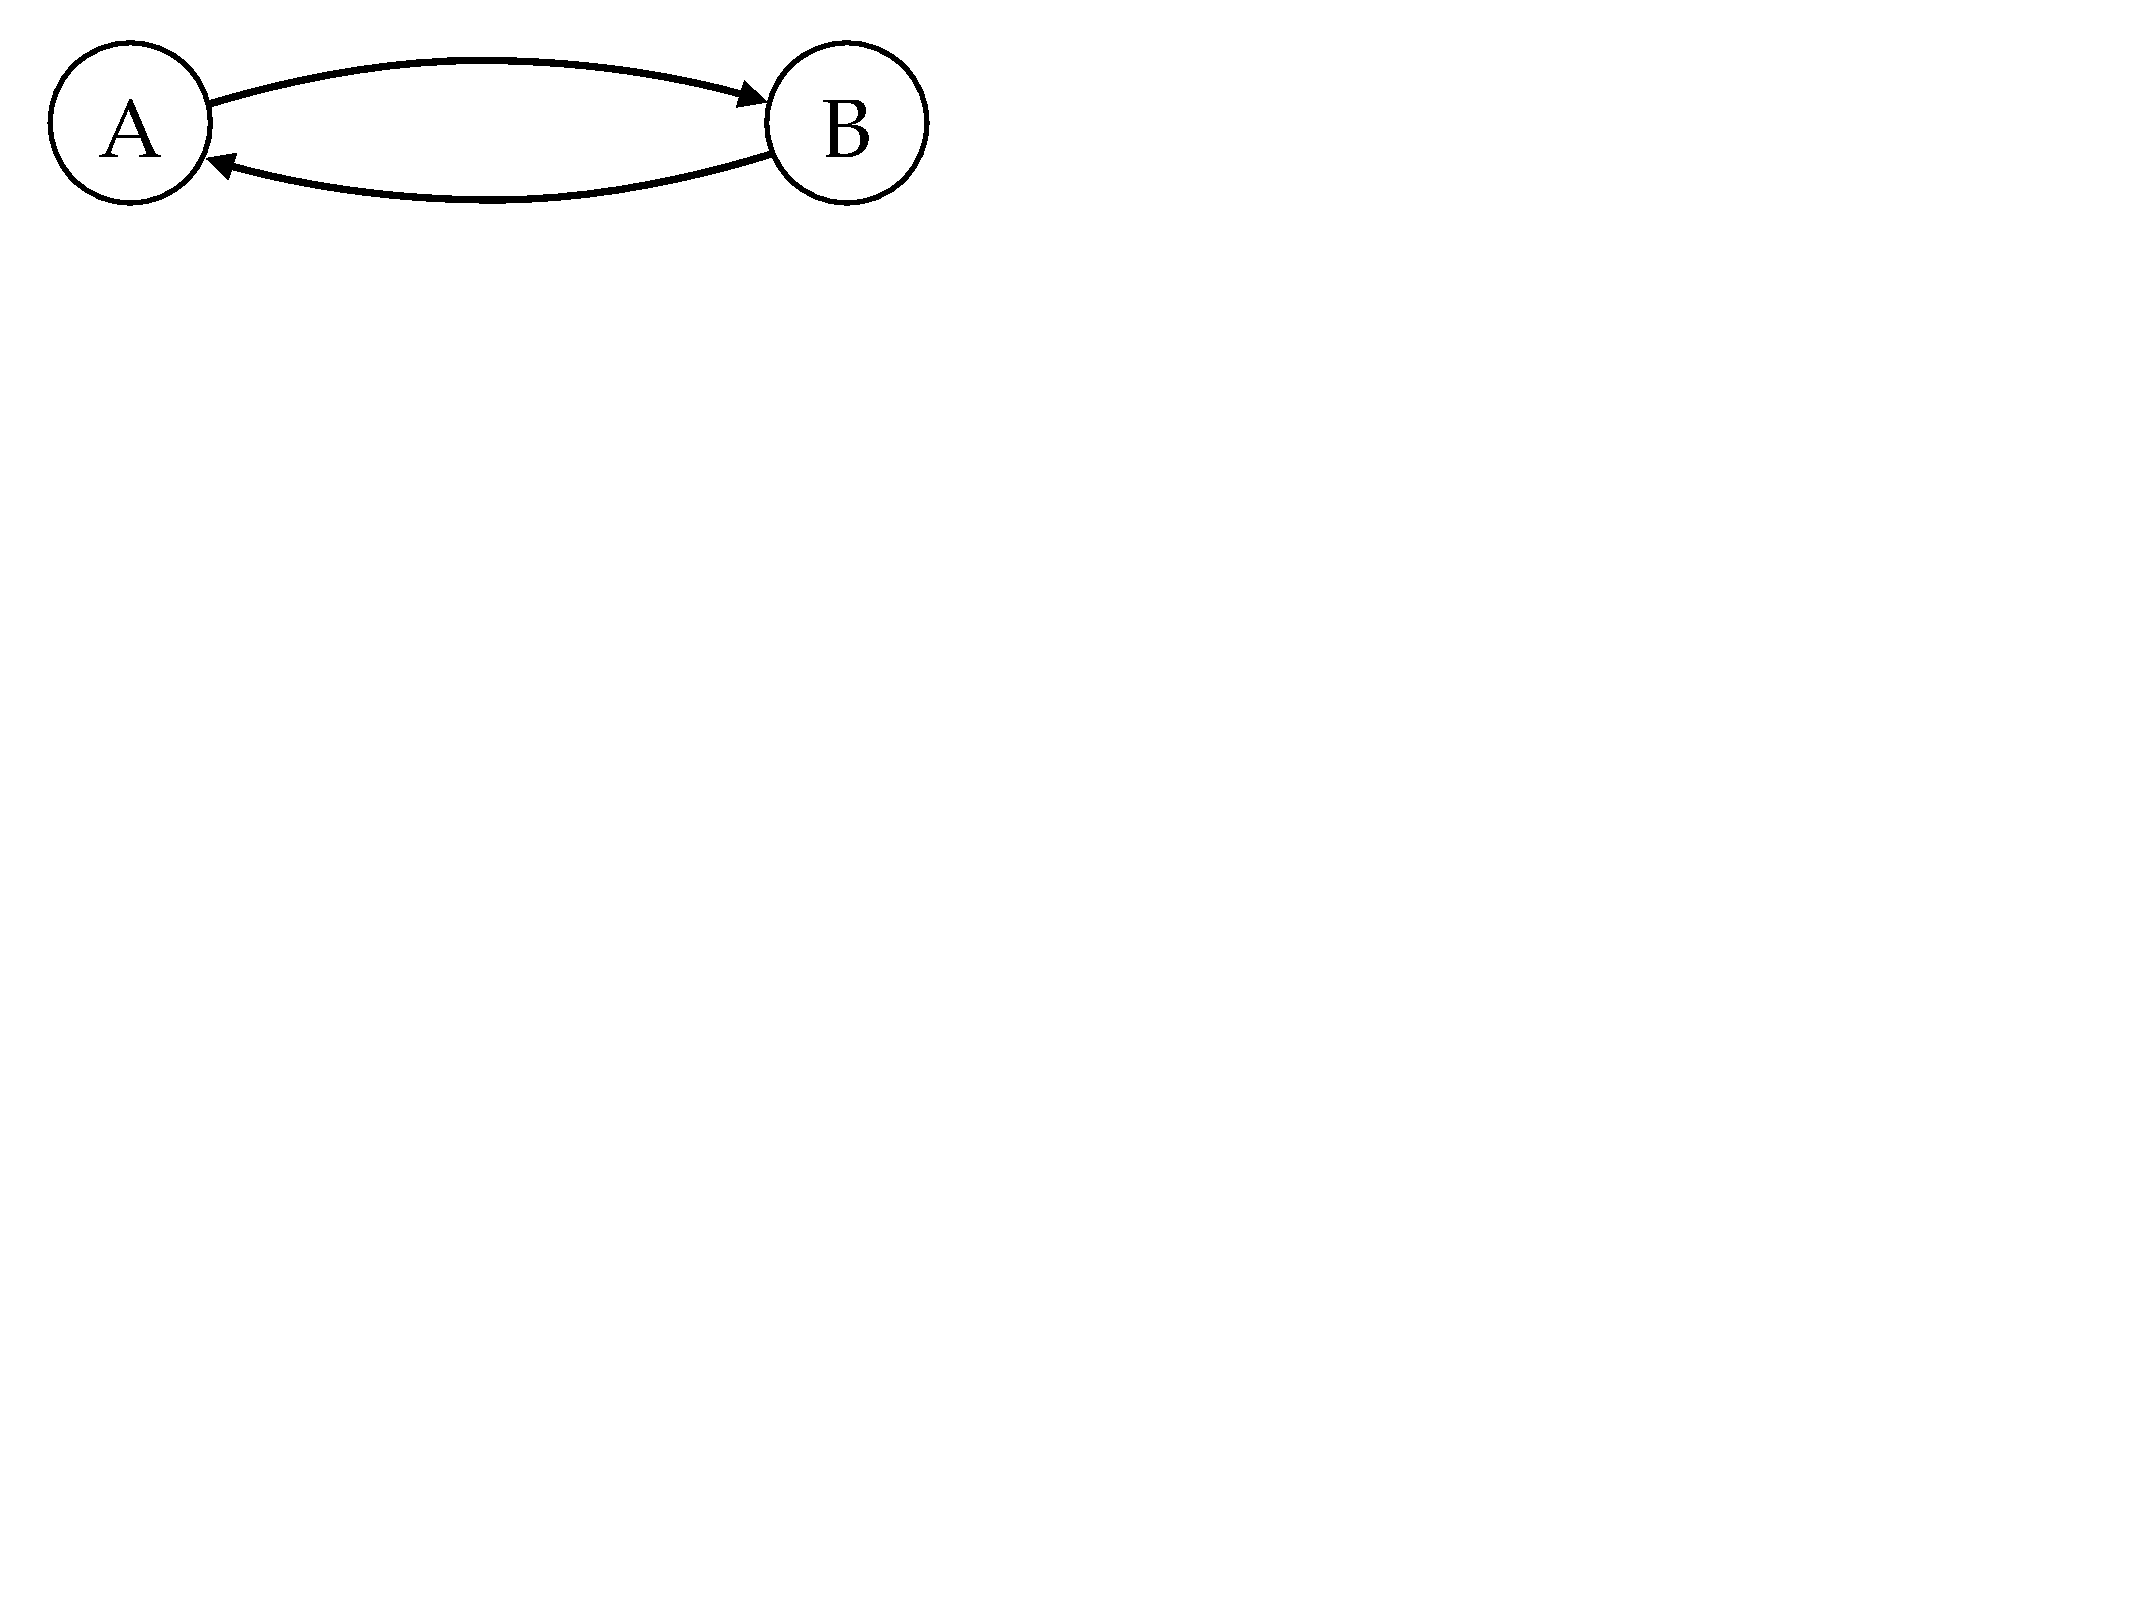
\includegraphics[width=0.3\textwidth]{cycle.pdf}
    \caption{The simplest cyclic directed graph. \figlabel{cycle}}
\end{figure}

% === Problem 4 ===
\section{Problem 4}

We are given the three statements

\begin{enumerate}
    \item{\label{s1}$\pr{A,B|C} = \pr{A|C}\,\pr{B|C}$}
    \item{\label{s2}$\pr{A|B,C} = \pr{A|C}$}
    \item{\label{s3}$\pr{B|A,C} = \pr{B|C}$}
\end{enumerate}

\noindent To see that statement \ref{s1} implies statement \ref{s2}, apply
the chain rule to find
\begin{equation}
    \pr{A|C}\,\pr{B|C} \stackrel{1}{=} \pr{A,B|C} = \pr{B|C} \, \pr{A | B,C}.
\end{equation}
Cancelling \pr{B|C} on both sides, we find statement 2. Therefore, it is
clear that statement 1 implies statement 2. Also, since we have only used
the chain rule, the inverse also applies. Specifically, applying the chain
rule to statement 2, we find
\begin{equation}
    \pr{A|B,C} = \frac{\pr{A,B|C}}{\pr{B|C}} \stackrel{2}{=} \pr{A|C}
        \to [\mathrm{Statement}\,1].
\end{equation}
Similarly, statement 1 implies statement 3 as follows
\begin{equation}
    \pr{A|C}\,\pr{B|C} \stackrel{1}{=} \pr{A,B|C} = \pr{A|C} \, \pr{B|A,C}
        \to [\mathrm{Statement}\,3]
\end{equation}
and the inverse
\begin{equation}
    \pr{B|A,C} = \frac{\pr{A,B|C}}{\pr{A|C}} \stackrel{3}{=} \pr{B|C}
        \to [\mathrm{Statement}\,1].
\end{equation}
Finally, since the equivalence holds between 1 and 2 and also between 1 and 3,
it is clear that 2 and 3 are also equivalent.


% === Problem 5 ===
\section{Problem 5}

\paragraph{(a)}

By Bayes' Theorem,
\begin{equation}
    \eqlabel{p51}
    \pr{H | E_1,E_2} = \frac{\pr{E_1, E_2|H} \, \pr{H}}{\pr{E_1,E_2}}.
\end{equation}
Therefore, set (ii) is clearly sufficient for this calculation. Without any
conditional independence assumptions, \eq{p51} cannot be simplified any
further so the other two sets are not sufficient. In particular,
$\pr{E_1, E_2|H} \ne \pr{E_1|H}\,\pr{E_2|H}$ unless $E_1 \perp E_2 | H$.

\paragraph{(b)}

Since $E_1 \perp E_2 | H$, $\pr{E_1, E_2|H} = \pr{E_1|H}\,\pr{E_2|H}$ and
\eq{p51} becomes
\begin{equation}
    \pr{H | E_1,E_2} = \frac{\pr{E_1|H}\, \pr{E_2|H} \, \pr{H}}{\pr{E_1,E_2}}.
\end{equation}
Therefore, sets (i) and (ii) are now sufficient. Set (iii) is not sufficient
because it would require that $E_1 \perp E_2$ but $E_1$ and $E_2$ are only
\emph{conditionally} independent.

% === Problem 6 ===
\section{Problem 6}

Since the variables $x$, $y$ and $z$ are interchangeable in this
distribution, it is sufficient to show that none of the graphs in
\fig{gm2} imply the same set of independences as the distribution.
The joint distribution of $x$, $y$ and $z$ is
\begin{equation}
    \begin{array}{r|cccc}
        Z = & 0 & 0 & 1 & 1 \\
        X = & 0 & 1 & 0 & 1 \\\hline
        Y = 0 & 1/12 & 1/6 & 1/6 & 1/12 \\
            1 & 1/6 & 1/12 & 1/12 & 1/6 \\
    \end{array}
\end{equation}
The first graph in \fig{gm2} implies the condition $X \perp Z | Y$ or,
\begin{equation}
    p(X,Y,Z) = p(X) \, p(Y | X) \, p (Z | Y).
\end{equation}
For our example, $p(X=1) = 1/2$, $p(Y = 1 | X =1) = 1/2$ and
$p(Z = 1 | Y = 1) = 1/2$ while $p(X=1, Y=1, Z=1) = 1/6$ therefore,
\begin{equation}
    \frac{1}{6} \ne \frac{1}{2} \times \frac{1}{2} \times \frac{1}{2}.
\end{equation}

For the next graphs, it is important to note that $X$ and $Y$ are
independent, i.e.
\begin{equation}
    \pr{X, Y} \stackrel{?}{=} \pr{X} \, \pr{Y}
\end{equation}
where $\pr{X = 1} = 1/2$, $\pr{Y = 1} = 1/2$ and
$\pr{X=1,Y=1} = 1/4$ satisfy this equality.

The second graph in
\fig{gm2} also implies that
\begin{equation}
    \pr{X,Y,Z} = \pr{X} \, \pr{Y} \, \pr{Z | X,Y}
\end{equation}
but $\pr{Z = 1 | X = 1, Y = 1} = 2/3$ and $\pr{Z = 1, X = 1, Y = 1} = 1/6$
so this condition is not satisfied by the distribution.

For the third graph, the independence condition implied is
\begin{equation}
    \pr{X,Y,Z} = \pr{X} \, \pr{Y} \, \pr{Z | X}.
\end{equation}
We can try, for example, $\pr{Z = 1 | X = 1} = 1/4$ and
$\pr{X=1,Y=1,Z=1} = 1/6$. Therefore, this condition is not satisfied
since
\begin{equation}
    \frac{1}{6} \ne \frac{1}{2} \, \frac{1}{2} \, \frac{1}{4}.
\end{equation}

Finally, the fourth graph in \fig{gm2} is the easiest. It implies that this
distribution factors as
\begin{equation}
    \pr{X,Y,Z} = \pr{X} \, \pr{Y} \, \pr{Z}
\end{equation}
but \pr{X=1}, \pr{Y=1} and \pr{Z=1} are all equal to $1/2$ and
$\pr{X=1,Y=1,Z=1} = 1/6 \ne (1/2)^3$.

Therefore, since none of these graphs represent the same independences
as the distribution, no directed acyclic graph on 3 variables has
$I_\mathrm{d-sep} (G) = I(p)$.

\begin{figure}[hbtp]
    \centering
    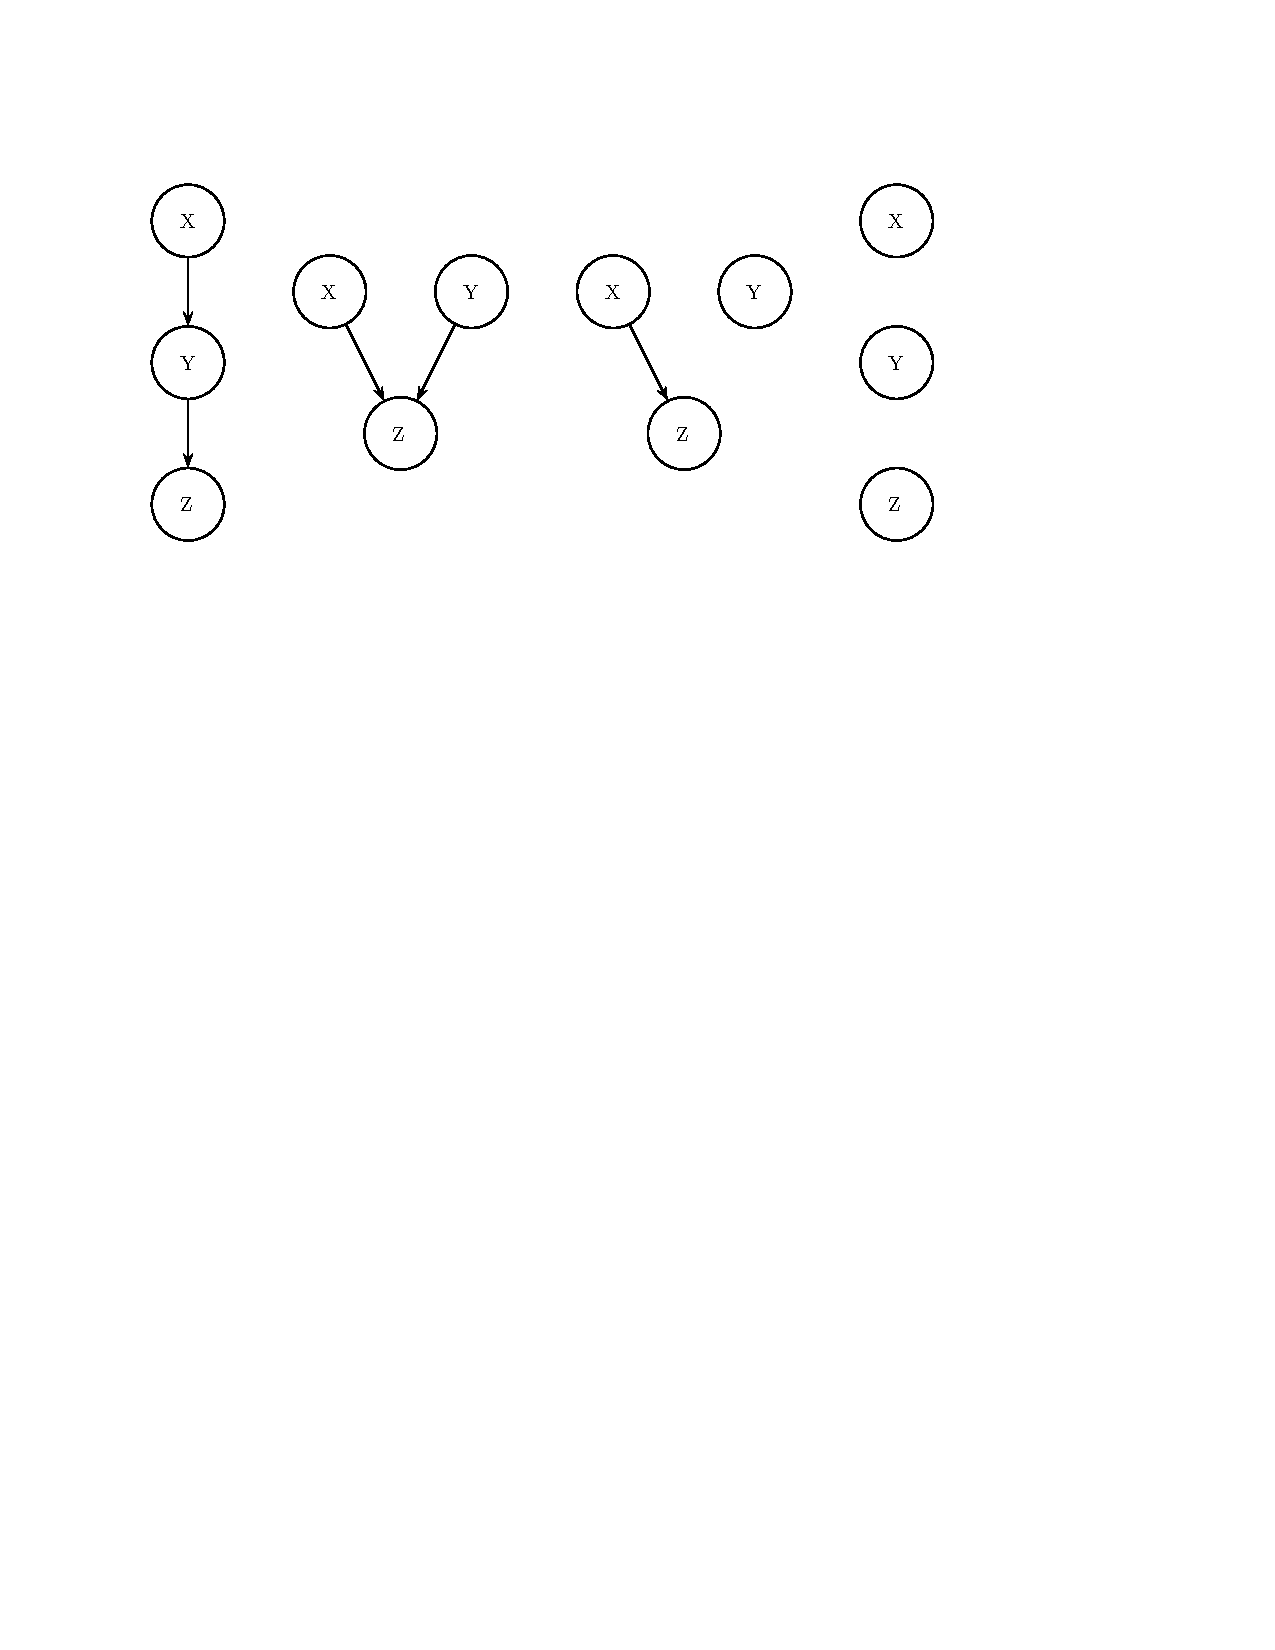
\includegraphics[width=0.8\textwidth,%
        trim=1.9cm 18cm 4.8cm 3cm,clip=true]{gm/gm2.pdf}
    \caption{The four different graphs on 3 random variables. \figlabel{gm2}}
\end{figure}

% === Problem 7 ===
\section{Problem 7}

\paragraph{(a) and (b)}

I will combine both parts for this question because I find it much easier
to generate the tables given a physical intuition.

\emph{Case 1:} $a > c$. The example for this one is that $X = 1$ means that
the fire alarm in your house is broken and it has a relatively small
prior probability $\pr{X=1} = 0.2$. Then, $Y=1$ indicates that there is
currently a fire in your house and $Z=1$ says that you can hear the fire
alarm going off. In this case, $\pr{X = 1|Z=1, Y=1} \sim 0$ because if the
fire alarm is going off \emph{and} there is a fire then the probability
that the alarm is broken is very small.

\emph{Case 2:} $a < c < b$. In this case, an example would be that
$X=1$ means that you are very intelligent, $Y = 1$ means that you
work very hard and $Z = 1$ means that you pass this class. There is
only a small prior probability that you are very intelligent ---
$\pr{X=1} = 0.1$ --- but if you pass then there is a higher
probability that you are very intelligent --- $\pr{X=1|Z=1} = 0.6$. In
between, if you pass but you're also a very hard worker, it's slightly
less likely that you're doing well based on your intelligence alone:
$\pr{X=1|Z=1,Y=1} = 0.5$.

\emph{Case 3:} $b < a < c$. A simple example satisfying this criterion is
that $Z = (X==Y)$. If the prior probability of $X=1$ is $\pr{X=1} = 0.5$
and the prior probability of $Y=1$ is $\pr{Y=1} = 0.01$ then,
$b = \pr{X=1|Z=1} = \pr{X=1|Z=1,Y=1}\pr{Y=1} + \pr{X=1|Z=1,Y=0}\pr{Y=0} = 0.01$
and $c = \pr{X=1|Z=1, Y=1} = 1$. The joint probability table is
\begin{equation}
    \begin{array}{r|cccc}
        Z =   & 0   & 0     & 1    & 1 \\
        X =   & 0   & 1     & 0    & 1 \\\hline
        Y = 0 & 0   & 0.495 & 0.495 & 0 \\
            1 & 0.005 & 0     & 0    & 0.005 \\
    \end{array}
\end{equation}

% === Problem 8 ===
\section{Problem 8}

\paragraph{(a)}

The set $A$ is $\{ X_2, X_3, X_4, X_5, X_8 \}$. Clearly, all the nodes
that are directly connected to $X_1$ (i.e.~$\{ X_2, X_3, X_4, X_8 \}$) must
be included in $A$ because a direct connection always constitutes an active
path. The inclusion of $X_5$ is not immediately obvious but if we just look
at the part of the graph containing $X_5$, we find the V-structure
$X_1 \to X_3 \gets X_5$. If we condition on $X_3$ (which we will do because
it is one of the directly connected nodes), it couples its parents $X_1$
and $X_5$.  Therefore, to satisfy the condition $X_1 \perp \chi-A-\{X_1\}|A$,
we must also include $X_5$ in $A$.  After the inclusion of $X_5$, there are
no other active paths between $X_1$ and other nodes outside of $A$ --- this
can be easily seen by trying them all.

\paragraph{(b)}

This algorithm generalizes as follows:
\begin{itemize}
    \item{Add all the children and parents of $X_i$ to $A$. As before,
        these are all required connections because any direct connection
        in the graph is an active path (i.e.~$X_i$ is never independent
        of these variables).}
    \item{This is not yet sufficient, however. If any of the children of
        $X_i$ (say $Y$) have other parents then conditioning on $Y$ couples
        $X_i$ to all of $Y$'s parents since it is a $V$-structure.
        Therefore, all of the parents of $Y$ must be added to $A$.}
    \item{This \emph{is} now sufficient because the neighbors of $X_i$'s
        parents and the children of $X_i$'s children are all
        conditionally independent of $X_i$, conditioned on $A$. This is
        easily seen by looking at the possible active paths in these
        directions and remembering that for a cascade structure, the
        end nodes are conditionally independent of each other conditioned
        on the middle node. This is also true for a common parent structure.}
\end{itemize}

% === Problem 9 ===
\section{Problem 9}

\paragraph{(a)}

Without any conditioning, the only (non-trivial) active paths in this graph
are: $1 \to 6 \to 4$, $8 \to 9 \to 5$, $4 \to 7 \to 9 \to 5$,
$4 \to 2 \to 10 \to 3 \to 9 \to 5$, $4 \to 6 \to 2 \to 10 \to 3 \to 9 \to 5$
and $6 \to 2 \to 4$.
Therefore, this implies the following set of independences:
$X_1 \perp X_2, X_3, X_5, X_7, X_8, X_9, X_{10}$, {$X_2 \perp X_1, X_7, X_8$}
{$X_3 \perp X_1, X_7, X_8$},
{$X_4 \perp X_8$},
{$X_5 \perp X_1$},
{$X_6 \perp X_7, X_8$},
{$X_7 \perp X_1, X_2, X_3, X_6, X_8, X_{10}$},
{$X_8 \perp X_1, X_2, X_3, X_4, X_6, X_7, X_{10}$},
{$X_9 \perp X_1$}, and
{$X_{10} \perp X_1, X_7, X_8$}. This can be more clearly summarized in the
following table:

\begin{equation}
    \begin{array}{c|cccccccccc}
            & 1     & 2     & 3     & 4     & 5     & 6     & 7     & 8     & 9     & 10     \\\hline
        1   &       & \perp & \perp &       & \perp &       & \perp & \perp & \perp & \perp  \\
        2   & \perp &       &       &       &       &       & \perp & \perp &       &        \\
        3   & \perp &       &       &       &       &       & \perp & \perp &       &        \\
        4   &       &       &       &       &       &       &       & \perp &       &        \\
        5   & \perp &       &       &       &       &       &       &       &       &        \\
        6   &       &       &       &       &       &       & \perp & \perp &       &        \\
        7   & \perp & \perp & \perp &       &       & \perp &       & \perp &       & \perp  \\
        8   & \perp & \perp & \perp & \perp &       & \perp & \perp &       &       & \perp  \\
        9   & \perp &       &       &       &       &       &       &       &       &        \\
        10  & \perp &       &       &       &       &       & \perp & \perp &       &        \\
    \end{array}
\end{equation}

\paragraph{(b)}

The conditioning on $\{ X_2, X_9 \}$ does not actually affect the set of
independences implied by the graph structure for $X_1$.  Therefore, the
largest set $A$ is $\{ X_3, X_5, X_7, X_8, X_{10} \}$.

\paragraph{(c)}

Using the $d$-separation algorithm from Koller~\&~Friedman, we find that the
only active paths (after conditioning on $\{ X_2, X_9 \}$) containing the node
$X_8$ are $8 \to 9 \to 3 \to 10 \to 2$ and $8 \to 9 \to 7 \to 4$.  Therefore,
the set $B$ is $\{ X_1, X_5, X_6 \}$.

% === Problem 10 ===
\section{Problem 10 --- Exercise 3.11}

\paragraph{(a)}

The left panel of \fig{gm3} shows graph from the problem and the right
panel shows the marginalized graph.

\paragraph{(b)}

The general procedure is as follows: to marginalize over a node $A$,
remove the node $A$ from the graph and draw edges directed from each
of the parents of $A$ to each of the children of $A$.

\paragraph{(c)}

Applying this procedure to the naive Bayes model and marginalizing
out the class variable will cause \emph{all} of the feature nodes to be
independent, i.e.~$X_i \perp \chi - \{ X_i \}$.

\begin{figure}[hbtp]
    \centering
    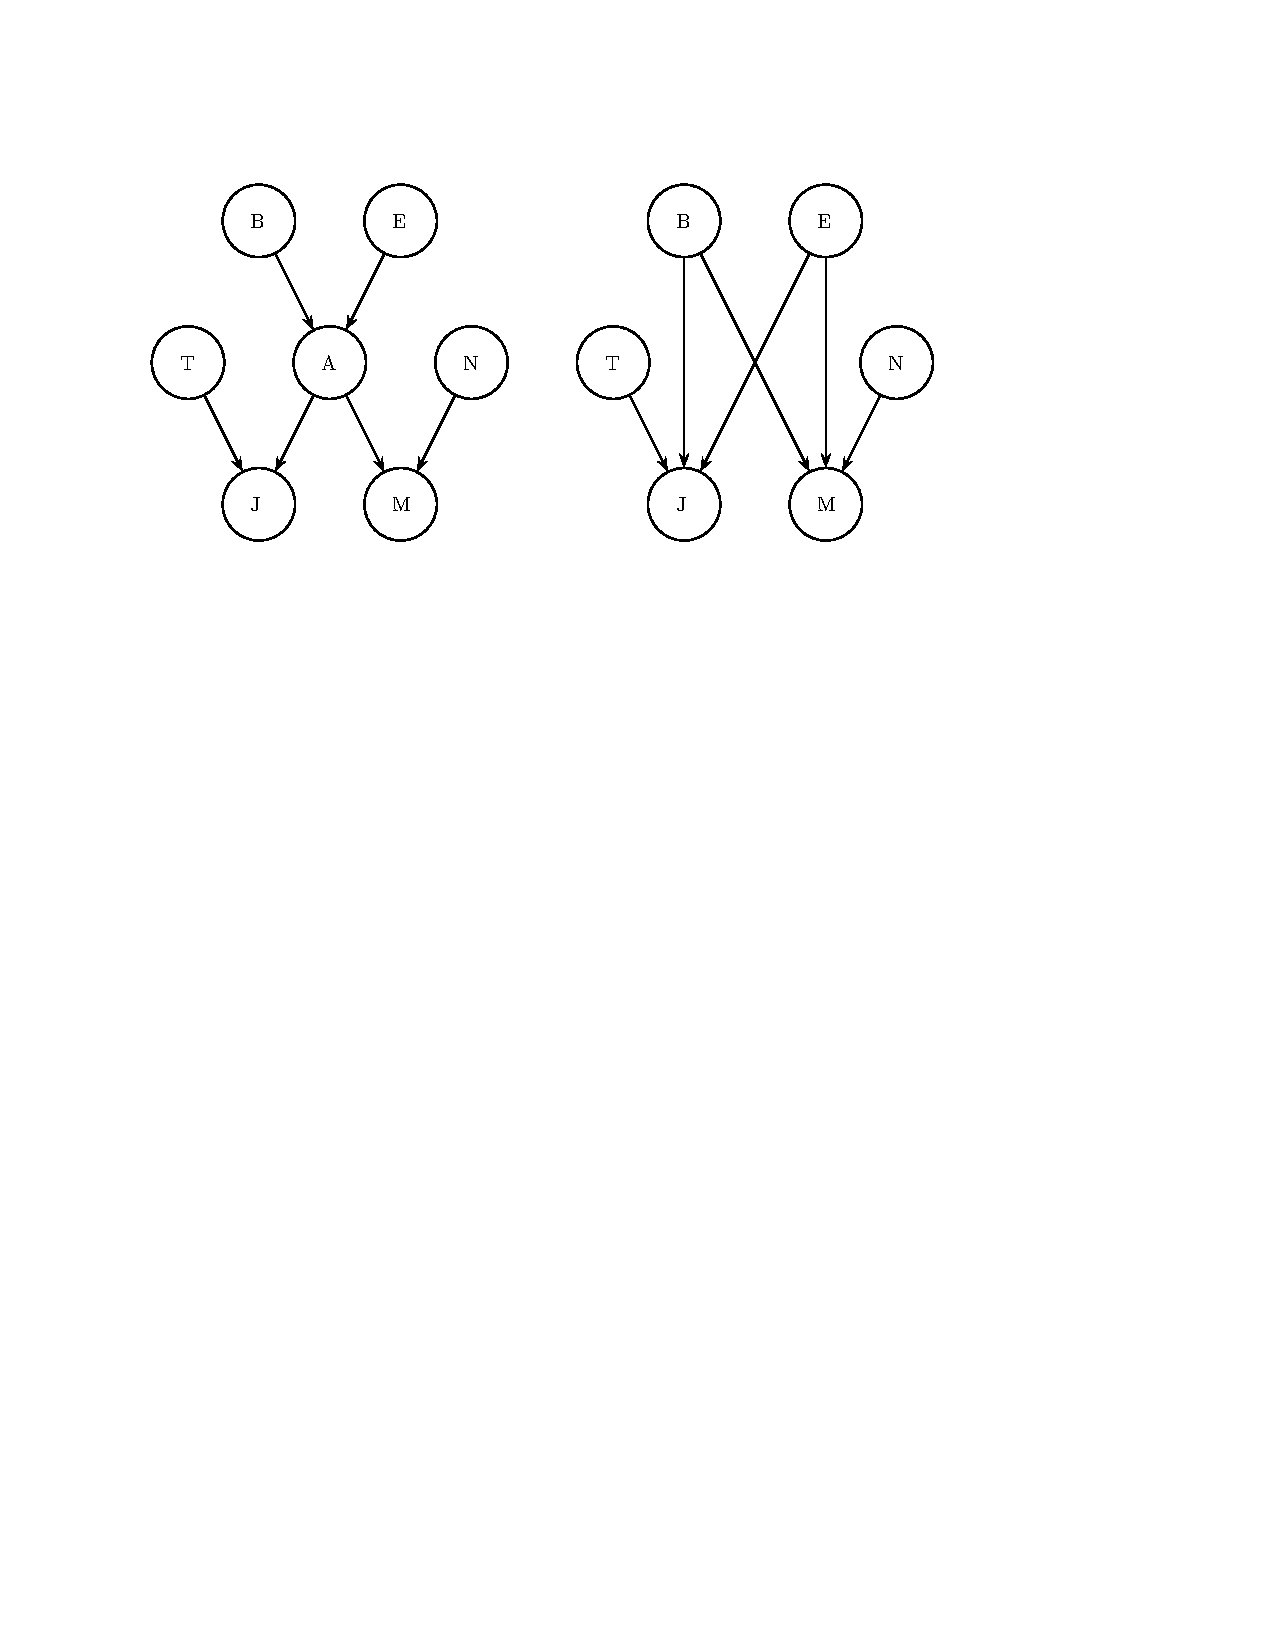
\includegraphics[width=0.8\textwidth,%
        trim=1.9cm 18cm 4.8cm 3cm,clip=true]{gm/gm3.pdf}
    \caption{\emph{Left}: the original graph. \emph{Right}: the graph
        marginalized over $A$.\figlabel{gm3}}
\end{figure}

% === Problem 11 ===
\section{Problem 11 --- Exercise 3.15}

The set of independences implied by graph (a) are $D \perp A,C | B$ and
$A \perp C$. There are no other $I$-equivalent graphs.
The independences implied by the Bayesian network (b) are $A \perp C,D|B$ and
$C \perp D | B$.  The four Bayesian networks (including (b) from the exercise)
in \fig{gm1} all imply this same independence structure. Therefore, they
are all $I$-equivalent.

\begin{figure}[hbtp]
    \centering
    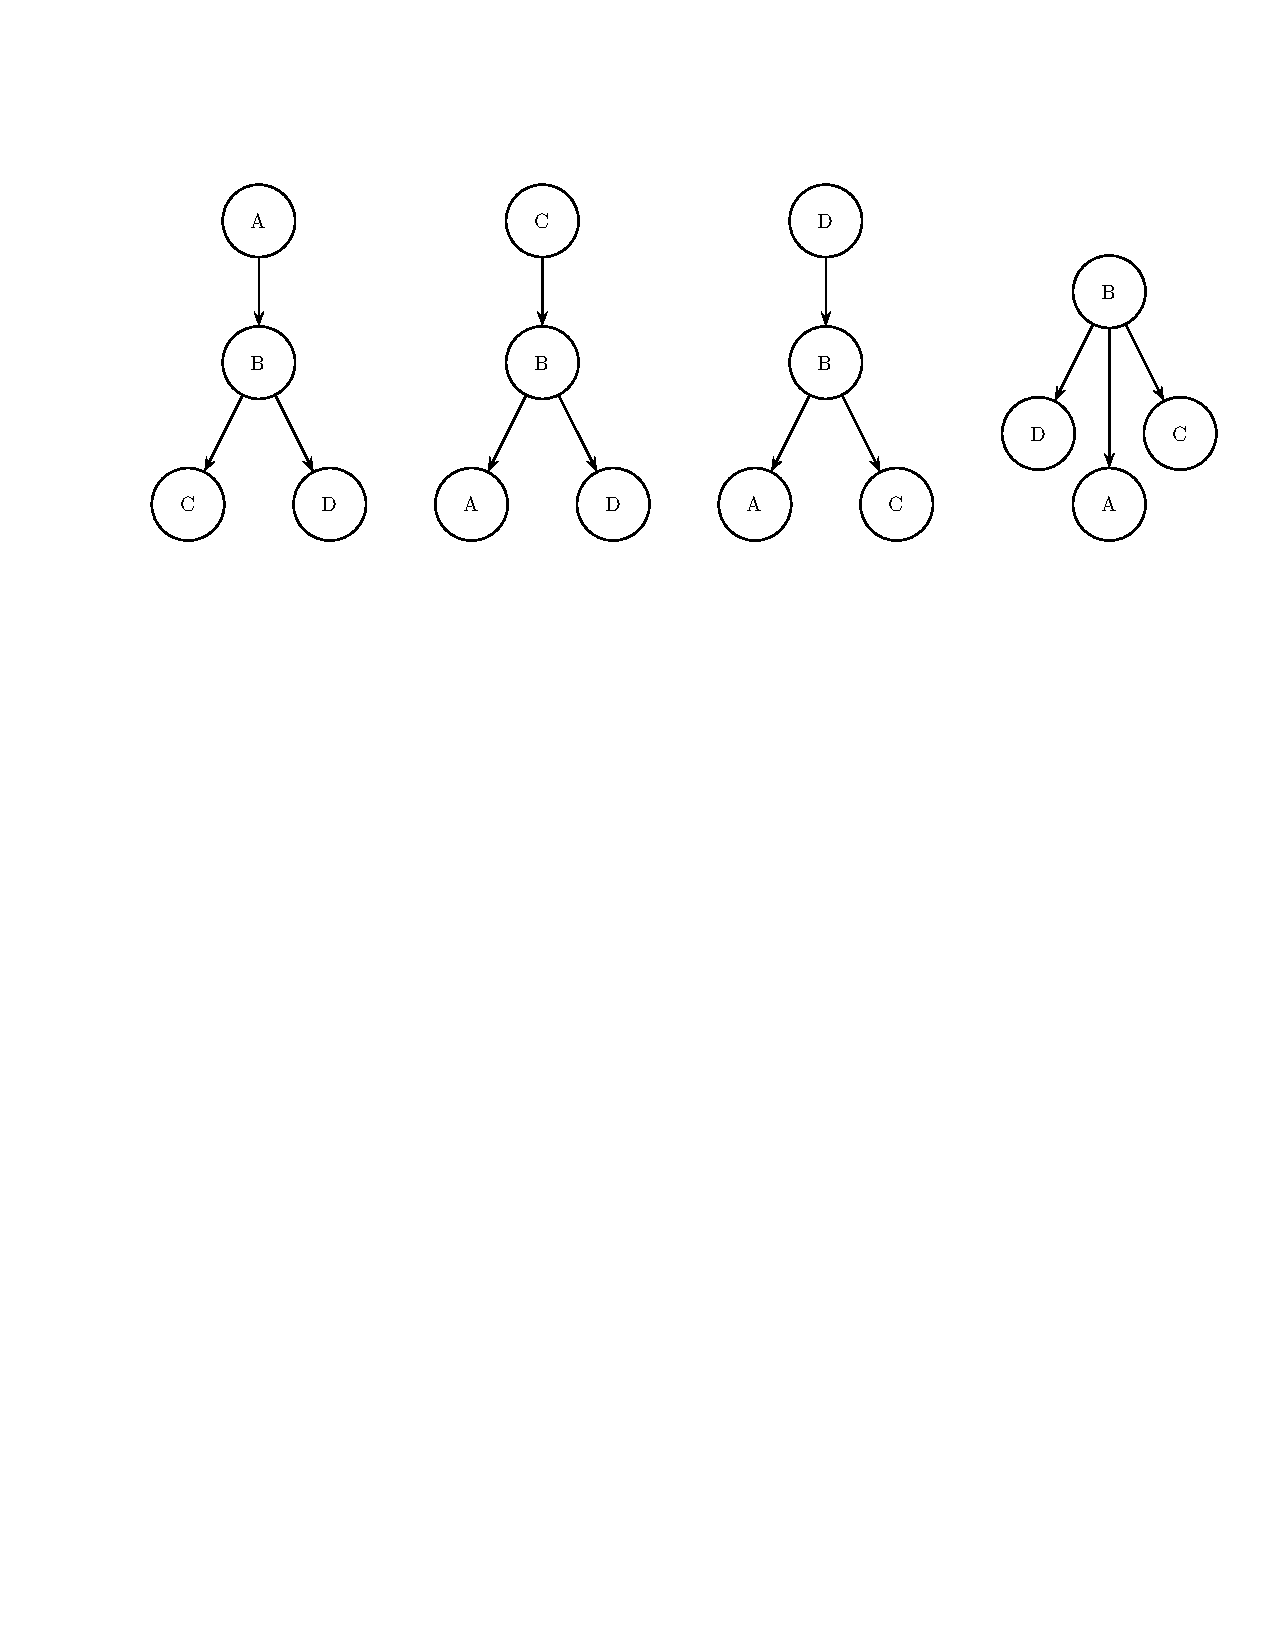
\includegraphics[width=0.8\textwidth,%
        trim=1.9cm 18cm 0.8cm 3cm,clip=true]{gm/gm1.pdf}
    \caption{Four $I$-equivalent Bayesian networks. \figlabel{gm1}}
\end{figure}

% === Problem 12 ===
\section{Problem 12 --- Exercise 3.2}

\paragraph{(a)}

The assumption given in Equation (3.6) is that each feature $X_i$ is
independent of the other features $\chi - \{X_i\}$ conditioned on the class
$C$. This can be written as $X_i \perp \chi - \{X_i\} | C$. Any joint
distribution $\pr{C, X_1, \ldots, X_n}$ can be factored (using the chain
rule) into $\pr{C} \, \pr{X_1, \ldots, X_n | C}$. Then, for a particular
feature $X_i$, the conditional independence assumption above implies that
\begin{equation}
    \pr{X_i, \chi-\{X_i\} | C} = \pr{X_i|C} \, \pr{\chi-\{X_i\} | C}.
\end{equation}
Applying the conditional independence assumption again, we find
\begin{equation}
    \pr{X_i|C} \, \pr{X_j, \chi-\{X_i, X_j\} | C}
        = \pr{X_i|C} \, \pr{X_j|C} \, \pr{\chi-\{X_i, X_j\} | C}.
\end{equation}
We can iterate this procedure for all values of $i = 1, \ldots, n$ to find
that
\begin{equation}
    \pr{X_1, \ldots, X_n | C} = \prod_{i=1}^{n} \pr{X_i | C}.
\end{equation}
Therefore, the conditional independence assumption from Equation (3.6)
implies that the join distribution can be factored
\begin{equation}\eqlabel{37}
    \pr{C, X_1, \ldots, X_n} = \pr{C} \, \prod_{i=1}^{n} \pr{X_i | C}
\end{equation}
which is exactly the result from Equation (3.7).

\paragraph{(b)}

Using the chain rule, we can rewrite the joint probability above as
\begin{equation}
    \pr{C,\bvec{X}} = \pr{\bvec{X}} \, \pr{C | \bvec{X}}.
\end{equation}
Therefore, the ratio of joint probabilities can be written (for the observed
feature vector \bvec{x})
\begin{equation}
    \frac{\pr{c_1, \bvec{x}}}{\pr{c_2, \bvec{x}}}
        = \frac{\pr{c_1 | \bvec{x}}}{\pr{c_2 | \bvec{x}}}.
\end{equation}
Then, using \eq{37}, this ratio can also be written
\begin{equation}
    \frac{\pr{c_1, \bvec{x}}}{\pr{c_2, \bvec{x}}} = \frac{\pr{c_1}}{\pr{c_2}}
        \prod_{i=1}^{n} \frac{\pr{x_i | c_1}}{\pr{x_i | c_2}}.
\end{equation}
Equating these two expressions, we find the expected Equation (3.8):
\begin{equation}\eqlabel{modcomp}
    \frac{\pr{c_1 | \bvec{x}}}{\pr{c_2 | \bvec{x}}}
    = \frac{\pr{c_1}}{\pr{c_2}}
        \prod_{i=1}^{n} \frac{\pr{x_i | c_1}}{\pr{x_i | c_2}}.
\end{equation}

\paragraph{(c)}

Taking the logarithm of \eq{modcomp}, we find
\begin{equation}
    \log \left [ \frac{\pr{c_1 | \bvec{x}}}{\pr{c_2 | \bvec{x}}} \right ]
        = \log \left [ \frac{\pr{c_1}}{\pr{c_2}} \right ] +
            \sum_{i=1}^n
            \left [ \log \pr{x_i | c_1} - \log \pr{x_i | c_2} \right ]
\end{equation}


% === Problem 13 ===
\section{Problem 13}

\paragraph{(a)}

A recursive equation for the marginalized probability $\pr{X_i = 1}$ is given
by
\begin{equation}\eqlabel{recurse}
    \pr{X_i=1} = \pr{X_{i-1} = 1}
        \, \left [ \pr{X_i =1 | X_{i-1} = 1}
            - \pr{X_i =1 | X_{i-1} = 0} \right ]
        + \pr{X_i =1 | X_{i-1} = 0}.
\end{equation}
Starting with
\begin{equation}
    \pr{X_2=1} = \pr{X_{1} = 1} \, \pr{X_2 =1 | X_1 = 1}
               + \pr{X_{1} = 0} \, \pr{X_2 =1 | X_1 = 0},
\end{equation}
where everything is known, we can iterate using \eq{recurse} to find
$\pr{X_i = 1}$ for each $i=1, \ldots, n$ in linear time. The pseudocode
for this algorithm is shown here:

\begin{lstlisting}

    # given px[i,1,1] = p(X[i] = 1 | X[i-1] = 1)
    # and px1[1] = p(X[1] = 1)

    pxi1 = []

    pxi1.push( px1[1] )

    for i in 2...n:
        pxi1.push( pxi1[-1] * (px[i,1,1] - px[i,1,0]) + px[i,1,0] )

    # now, pxi1 contains a list of all the p(X[i] = 1)

\end{lstlisting}

\paragraph{(b)}

Analogous to \eq{recurse}, the recursive form for the conditional
probability is
\begin{equation*}
    \pr{X_i=1 | X_1 = 1} =
        \pr{X_{i-1} = 1 | X_1 = 1}
        \, \left [ \pr{X_i =1 | X_{i-1} = 1}
            - \pr{X_i =1 | X_{i-1} = 0} \right ]
        + \pr{X_i =1 | X_{i-1} = 0}.
\end{equation*}
and the algorithm is

\begin{lstlisting}

    pxi1 = []

    pxi1.push( px[2,1,1] )

    for i in 3...n:
        pxi1.push( pxi1[-1] * (px[i,1,1] - px[i,1,0]) + px[i,1,0] )

    # now, pxi1 contains a list of all the p(X[i] = 1 | X[1] = 1)

\end{lstlisting}

\paragraph{(c)}

By Bayes,
\begin{equation}
    \pr{X_1 = 1 | X_i = 1} =
        \frac{\pr{X_1 = 1} \, \pr{X_i = 1 | X_1 = 1}}{\pr{X_i=1}}
\end{equation}
Therefore, the algorithm becomes
\begin{lstlisting}

    px = []

    pxi1  = px1[1] * (px[2,1,1] - px[2,1,0]) + px[2,1,0]
    pcond = px[2,1,1]

    px.push( px1[1] * pcond / pxi1 )

    for i in 3...n:
        pxi1  = pxi1  * (px[i,1,1] - px[i,1,0]) + px[i,1,0]
        pcond = pcond * (px[i,1,1] - px[i,1,0]) + px[i,1,0]
        px.push( px1[1] * pcond / pxi1 )

    # now, pxi1 contains a list of all the p(X[1] = 1 | X[i] = 1)

\end{lstlisting}
This still scales linearly with $n$.

\end{document}

